% Chapter Template

\chapter{Ensayos y resultados} % Main chapter title

\label{Chapter4} % Change X to a consecutive number; for referencing this chapter elsewhere, use \ref{ChapterX}

%----------------------------------------------------------------------------------------
%	SECTION 1
%----------------------------------------------------------------------------------------

En este capítulo se detallan los ensayos realizados para comprobar el correcto funcionamiento del firmware, hardware y pruebas de campo.
\section{Ensayo de firmware}
Para comprobar el correcto funcionamiento se realizaron los siguientes ensayos sobre algunas de las funciones que forman parte del firmware.
\subsection{Ensayo función clima}
Se envió la trama \$CON\# a través de la comunicación UDP. EL resultado de este ensayo se muestra en la figura \ref{fig: ensayo clima 1}. En la figura se observa el despligue de dos imágenes del agendamiento y las imágenes del clima. Las imágenes del clima se muestran durante cuatro segundos. En el archivo CONFIGURACION.csv se modificó el campo flagclima como se muestra en la figura \ref{fig: ensayo clima 2}. Cuando el sistema era reiniciado el firmware recuperaba la ultima configuración del campo flagclima como se muestra en la figura \ref{fig: ensayo clima 3}. 

\begin{figure}[htpb]
	\centering
	\includegraphics[scale=0.8]{Figures/pruebaclima1.png} 
	\caption{Ensayo habilitación función clima.}
	\label{fig: ensayo clima 1}
\end{figure}

\begin{figure}[htpb]
	\centering
	\includegraphics[scale=0.8]{Figures/pruebaclima2.png} 
	\caption{Configuración de clima activo.}
	\label{fig: ensayo clima 2}
\end{figure}

\begin{figure}[htpb]
	\centering
	\includegraphics[scale=0.8]{Figures/pruebaclima3.png} 
	\caption{Recuperación de ultimo estado de el campo flagclima.}
	\label{fig: ensayo clima 3}
\end{figure}

Se envió la trama \$COFF\# a través de la comunicación UDP.  EL resultado de este ensayo se muestra en la figura \ref{fig: pruebas clima 2}. En la figura se observa que las imágenes que corresponden al clima ya no aparecen.

\begin{figure}[htpb]
	\centering
	\includegraphics[scale=0.8]{Figures/prubasclimaoff.png} 
	\caption{Ensayo deshabilitación función clima.}
	\label{fig: pruebas clima 2}
\end{figure}

\subsection{Ensayo función reloj}

Se envió la trama \$HON\# a través de la comunicación UDP. EL resultado de este ensayo se muestra en la figura \ref{fig: ensayo reloj 1}. En la figura se observa el despligue de dos imágenes del agendamiento y las imágenes del reloj. Las imágenes del reloj se muestran durante cuatro segundos. En el archivo CONFIGURACION.csv se modificó el campo flagclock como se muestra en la figura \ref{fig: ensayo reloj 2}. Cuando el sistema era reiniciado el firmware recuperaba la ultima configuración del campo flagclock como se muestra en la figura \ref{fig: ensayo reloj 3}. 

\begin{figure}[htpb]
	\centering
	\includegraphics[scale=0.8]{Figures/pruebareloj1.png} 
	\caption{Ensayo habilitación función reloj.}
	\label{fig: ensayo reloj 1}
\end{figure}

\begin{figure}[htpb]
	\centering
	\includegraphics[scale=0.8]{Figures/pruebareloj2.png} 
	\caption{Configuración de reloj activo.}
	\label{fig: ensayo reloj 2}
\end{figure}

\begin{figure}[htpb]
	\centering
	\includegraphics[scale=0.8]{Figures/pruebaclima3.png} 
	\caption{Recuperación de ultimo estado de el campo flagclock.}
	\label{fig: ensayo reloj 3}
\end{figure}

Se envió la trama \$HOFF\# a través de la comunicación UDP.  EL resultado de este ensayo se muestra en la figura \ref{fig: pruebas clima 2}. En la figura se observa que las imágenes que corresponden al reloj ya no aparecen.

\begin{figure}[htpb]
	\centering
	\includegraphics[scale=0.8]{Figures/pruebareloj4.png} 
	\caption{Ensayo deshabilitación función reloj.}
	\label{fig: ensayo reloj 4}
\end{figure}




\section{Ensayo de hardware}
\subsection{PCB matriz de LEDs}
Para comprobar el correcto funcionamiento de las matrices de LEDs se armó un banco de pruebas de matrices de LEDs con el cual se pudo comprobar el correcto funcionamiento de las matrices de LEDs. El prototipo de prueba de matrices de LEDs enciende los colores básico (rojo, verde y azul ) y realiza secuencias básicas. Con este banco se comprobó el correcto funcionamiento de las PCBs matriz de LEDs. En la figura \ref{fig: banco de pruebas} se muestra personal de la empresa realizando el  test de calidad utilizando el banco de pruebas para descartar errores de soldadura.

\begin{figure}[htpb]
	\centering
	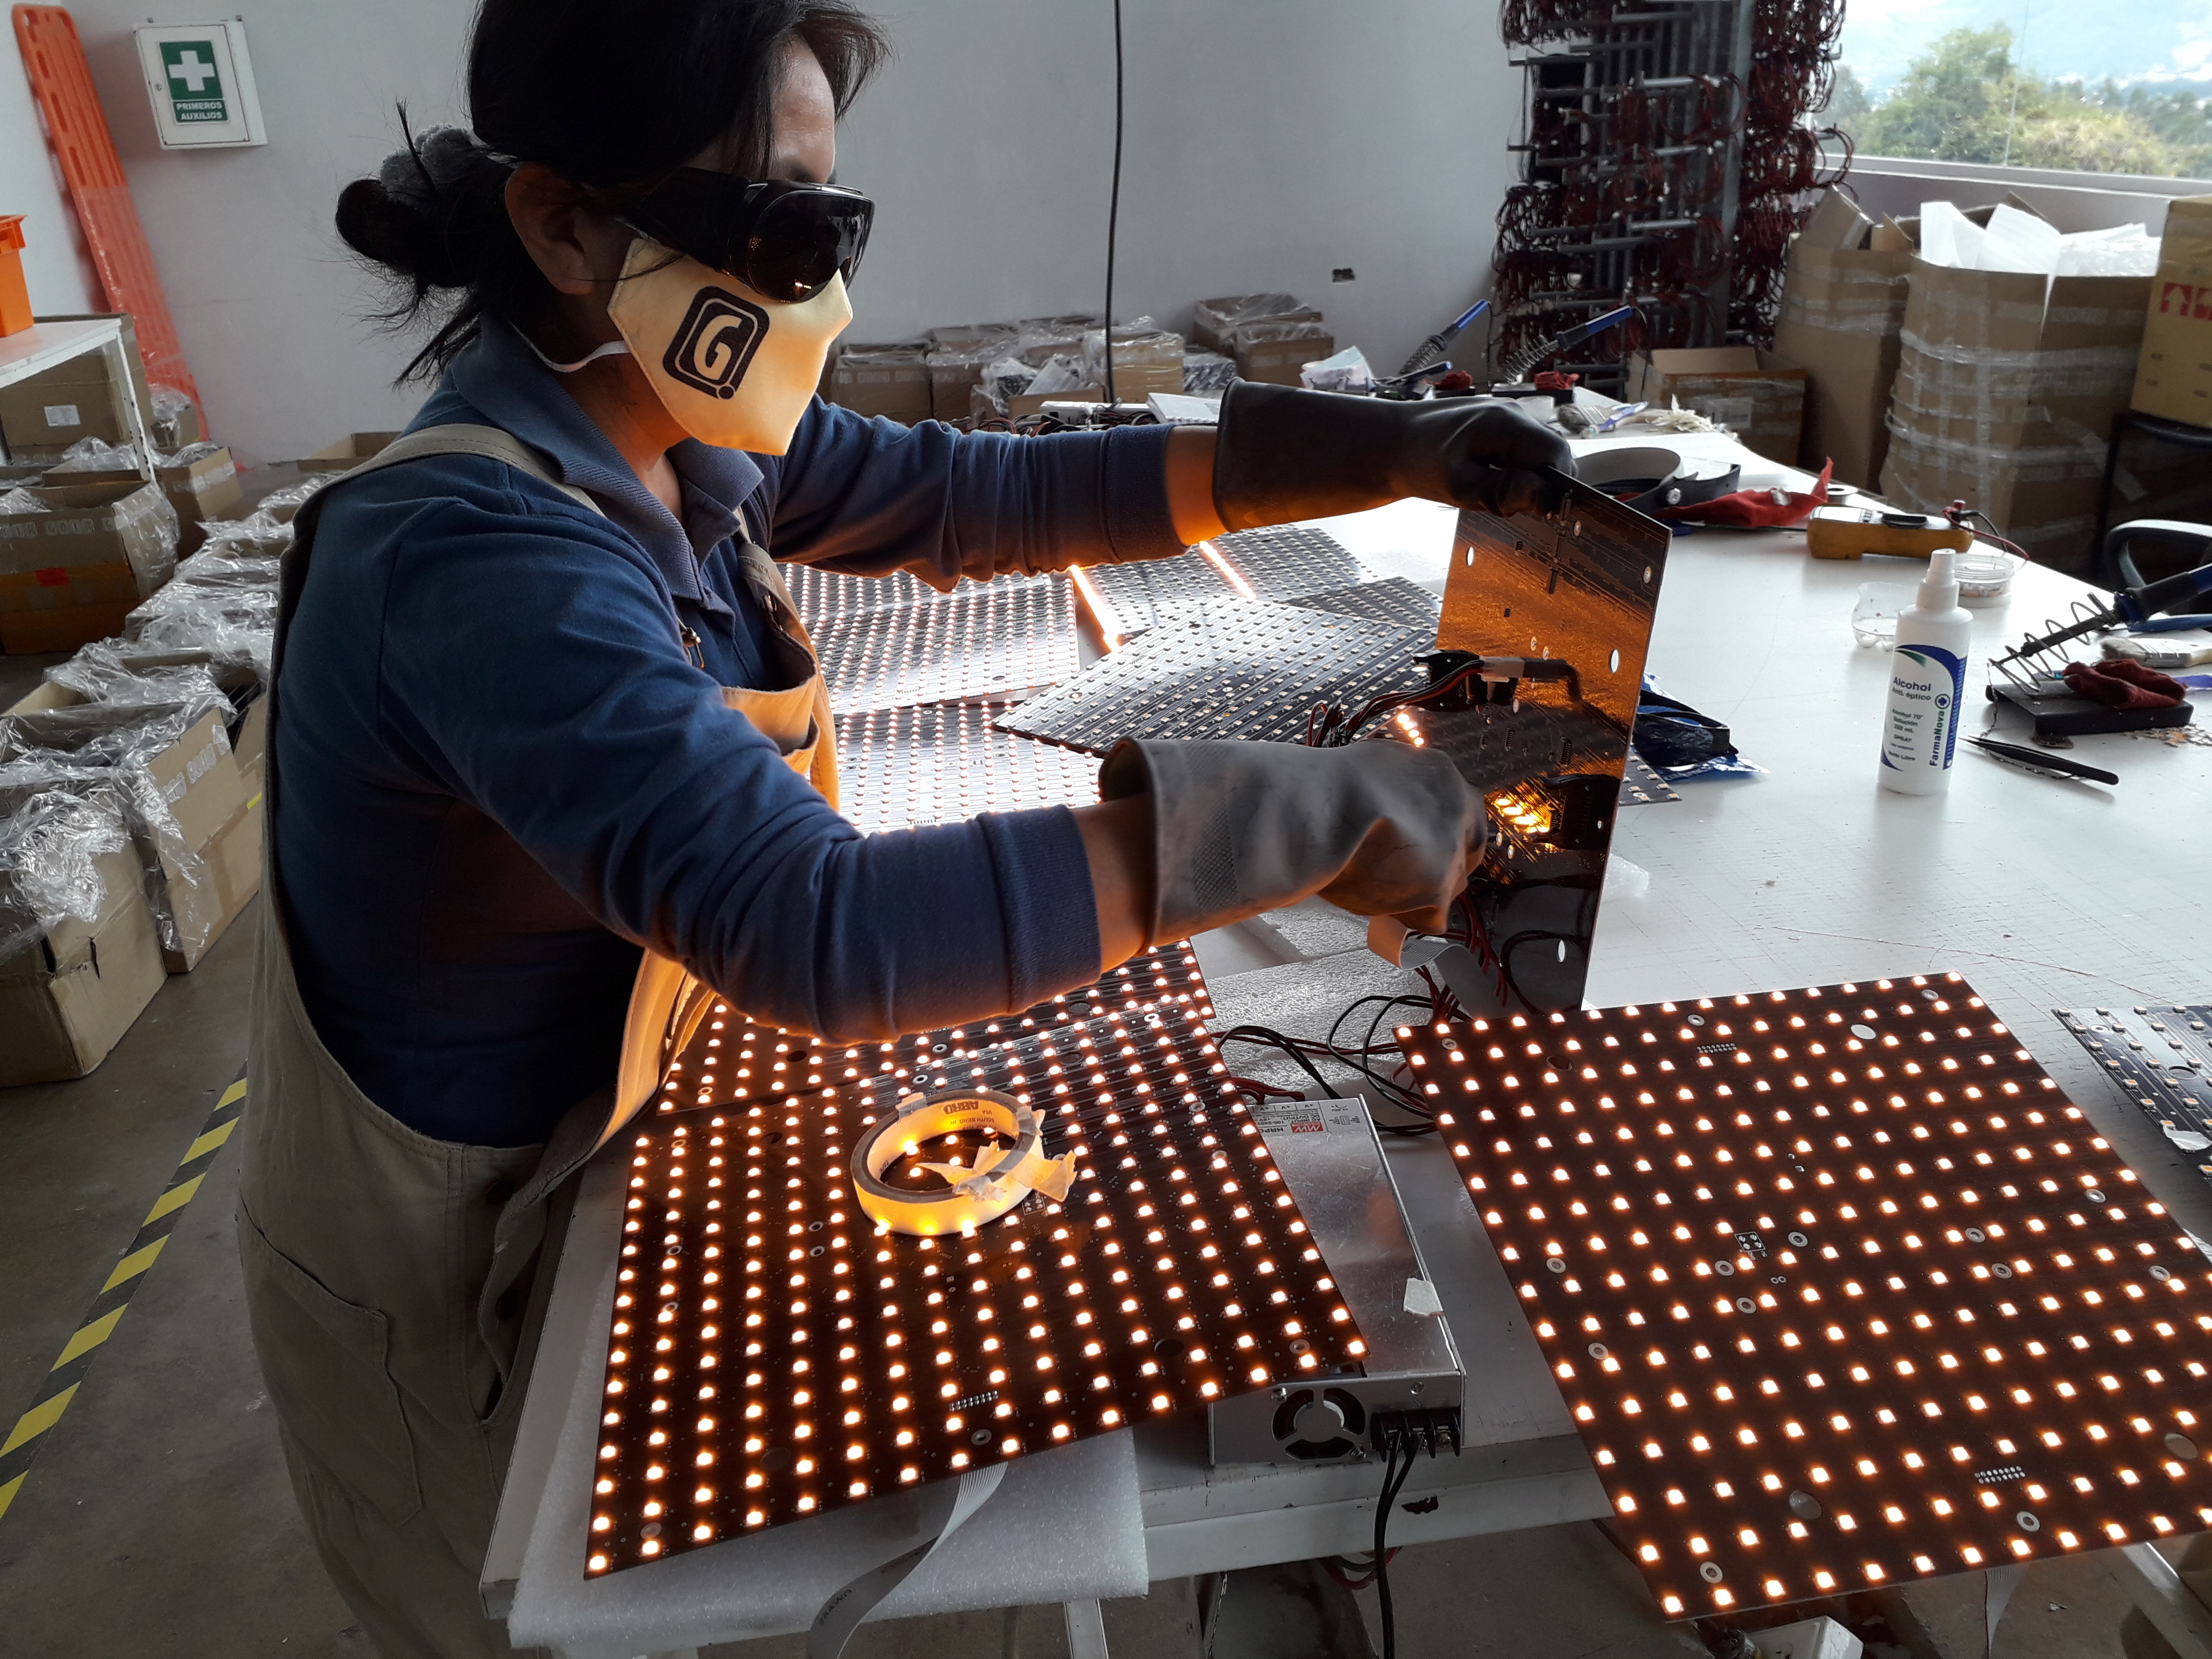
\includegraphics[scale=0.1]{Figures/testmatrices.jpg} 
	\caption{Banco de pruebas.}
	\label{fig: banco de pruebas}
\end{figure}



\subsection{PCB matriz de distribución}
Para comprobar el correcto funcionamiento de la PCB se colocó una señal cuadrada en al entrada del PCB y se observó la señal de salida con un osciloscopio. Los resultados de este ensayo se muestran en la figura \ref{fig: capturaosciloscopio}. Se observa la señal de entrada en el canal uno y la señal de salida en el canal 2. La frecuencia de las dos señales es 2,5 MHz. La amplitud de la señal de entrada es de 3,3 V y la amplitud de la señal de salida es de 5 V. 

\begin{figure}[htpb]
	\centering
	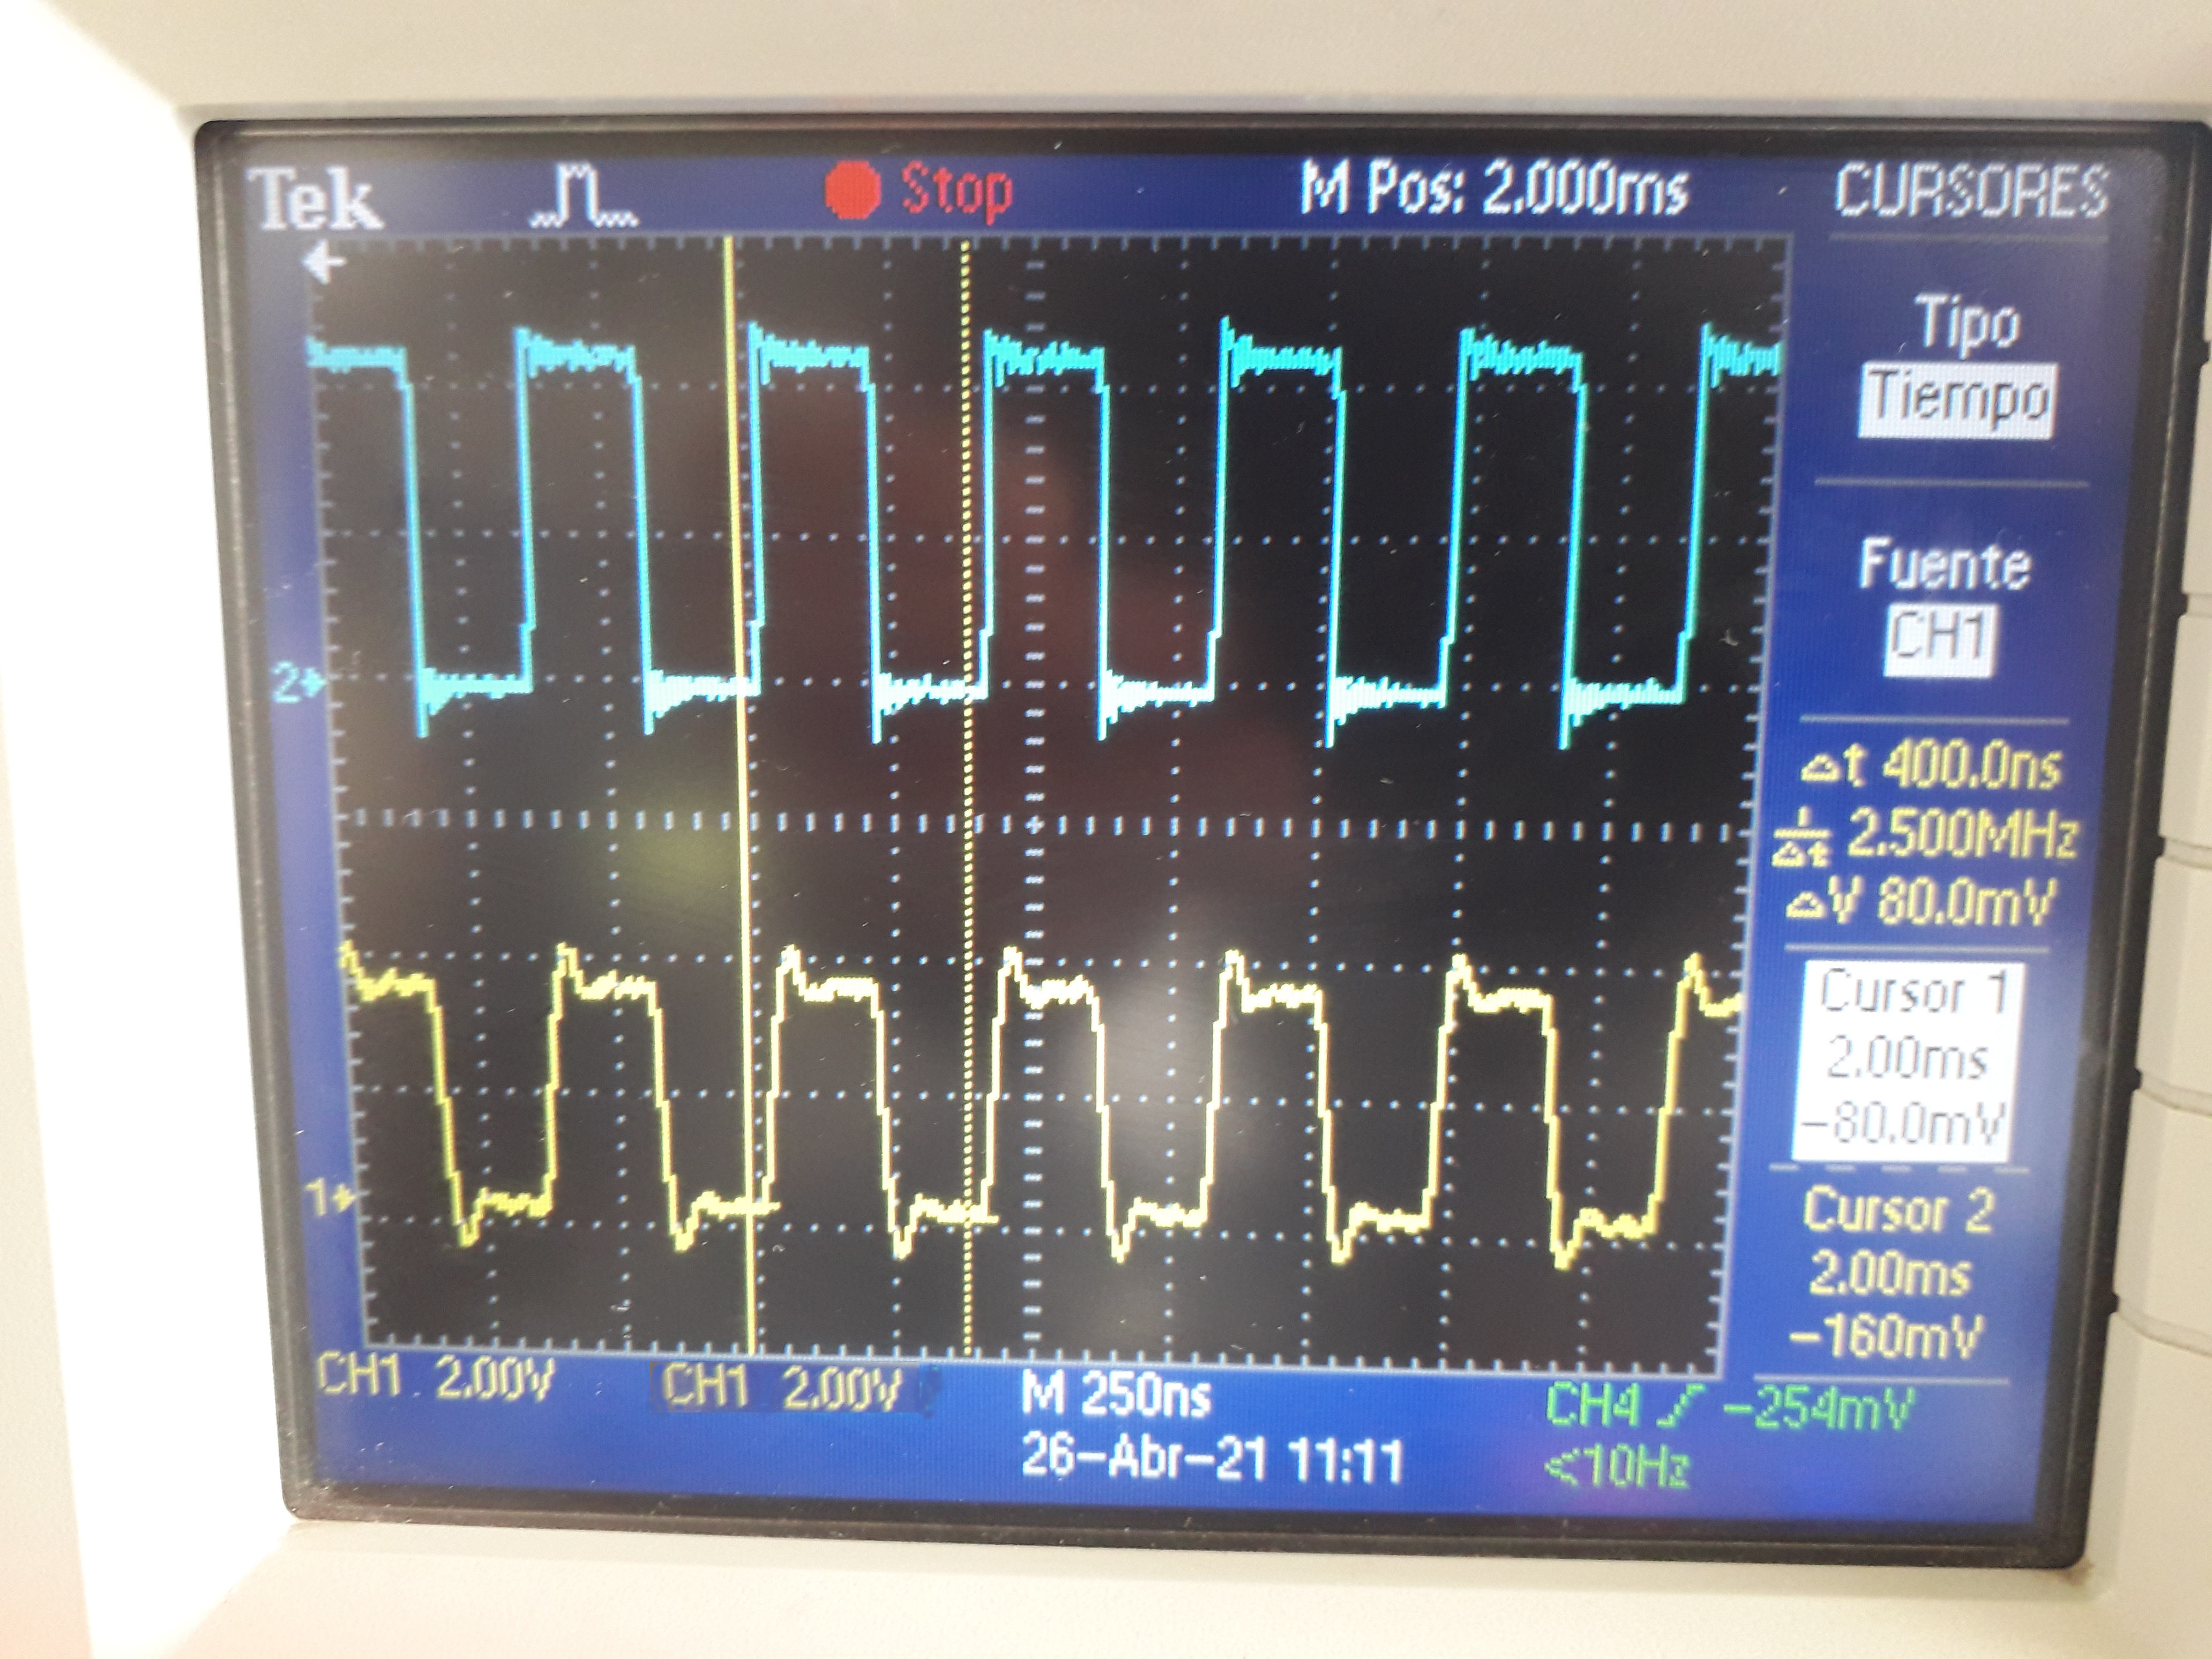
\includegraphics[scale=0.1]{Figures/osciloscopio.jpg} 
	\caption{Pruebas de PCB de distribución con osciloscopio.}
	\label{fig: capturaosciloscopio}
\end{figure}




\section{Ensayo de sistema}
\subsection{Ensayo de matrices sobre mesa de trabajo}
Este ensayo se la realizó armando el prototipo sobre una mesa de pruebas. Se cargaron las imágenes en la carpeta compartida y se corrió el firmware a través de la consola de comandos. Los resultados de esta prueba se los puede observar en la figura \ref{fig: matriz4x4}. Debido a el posicionamiento inadecuado y el angulo de visión de las PCBs no se puede apreciar la imagen.

\begin{figure}[htpb]
	\centering
	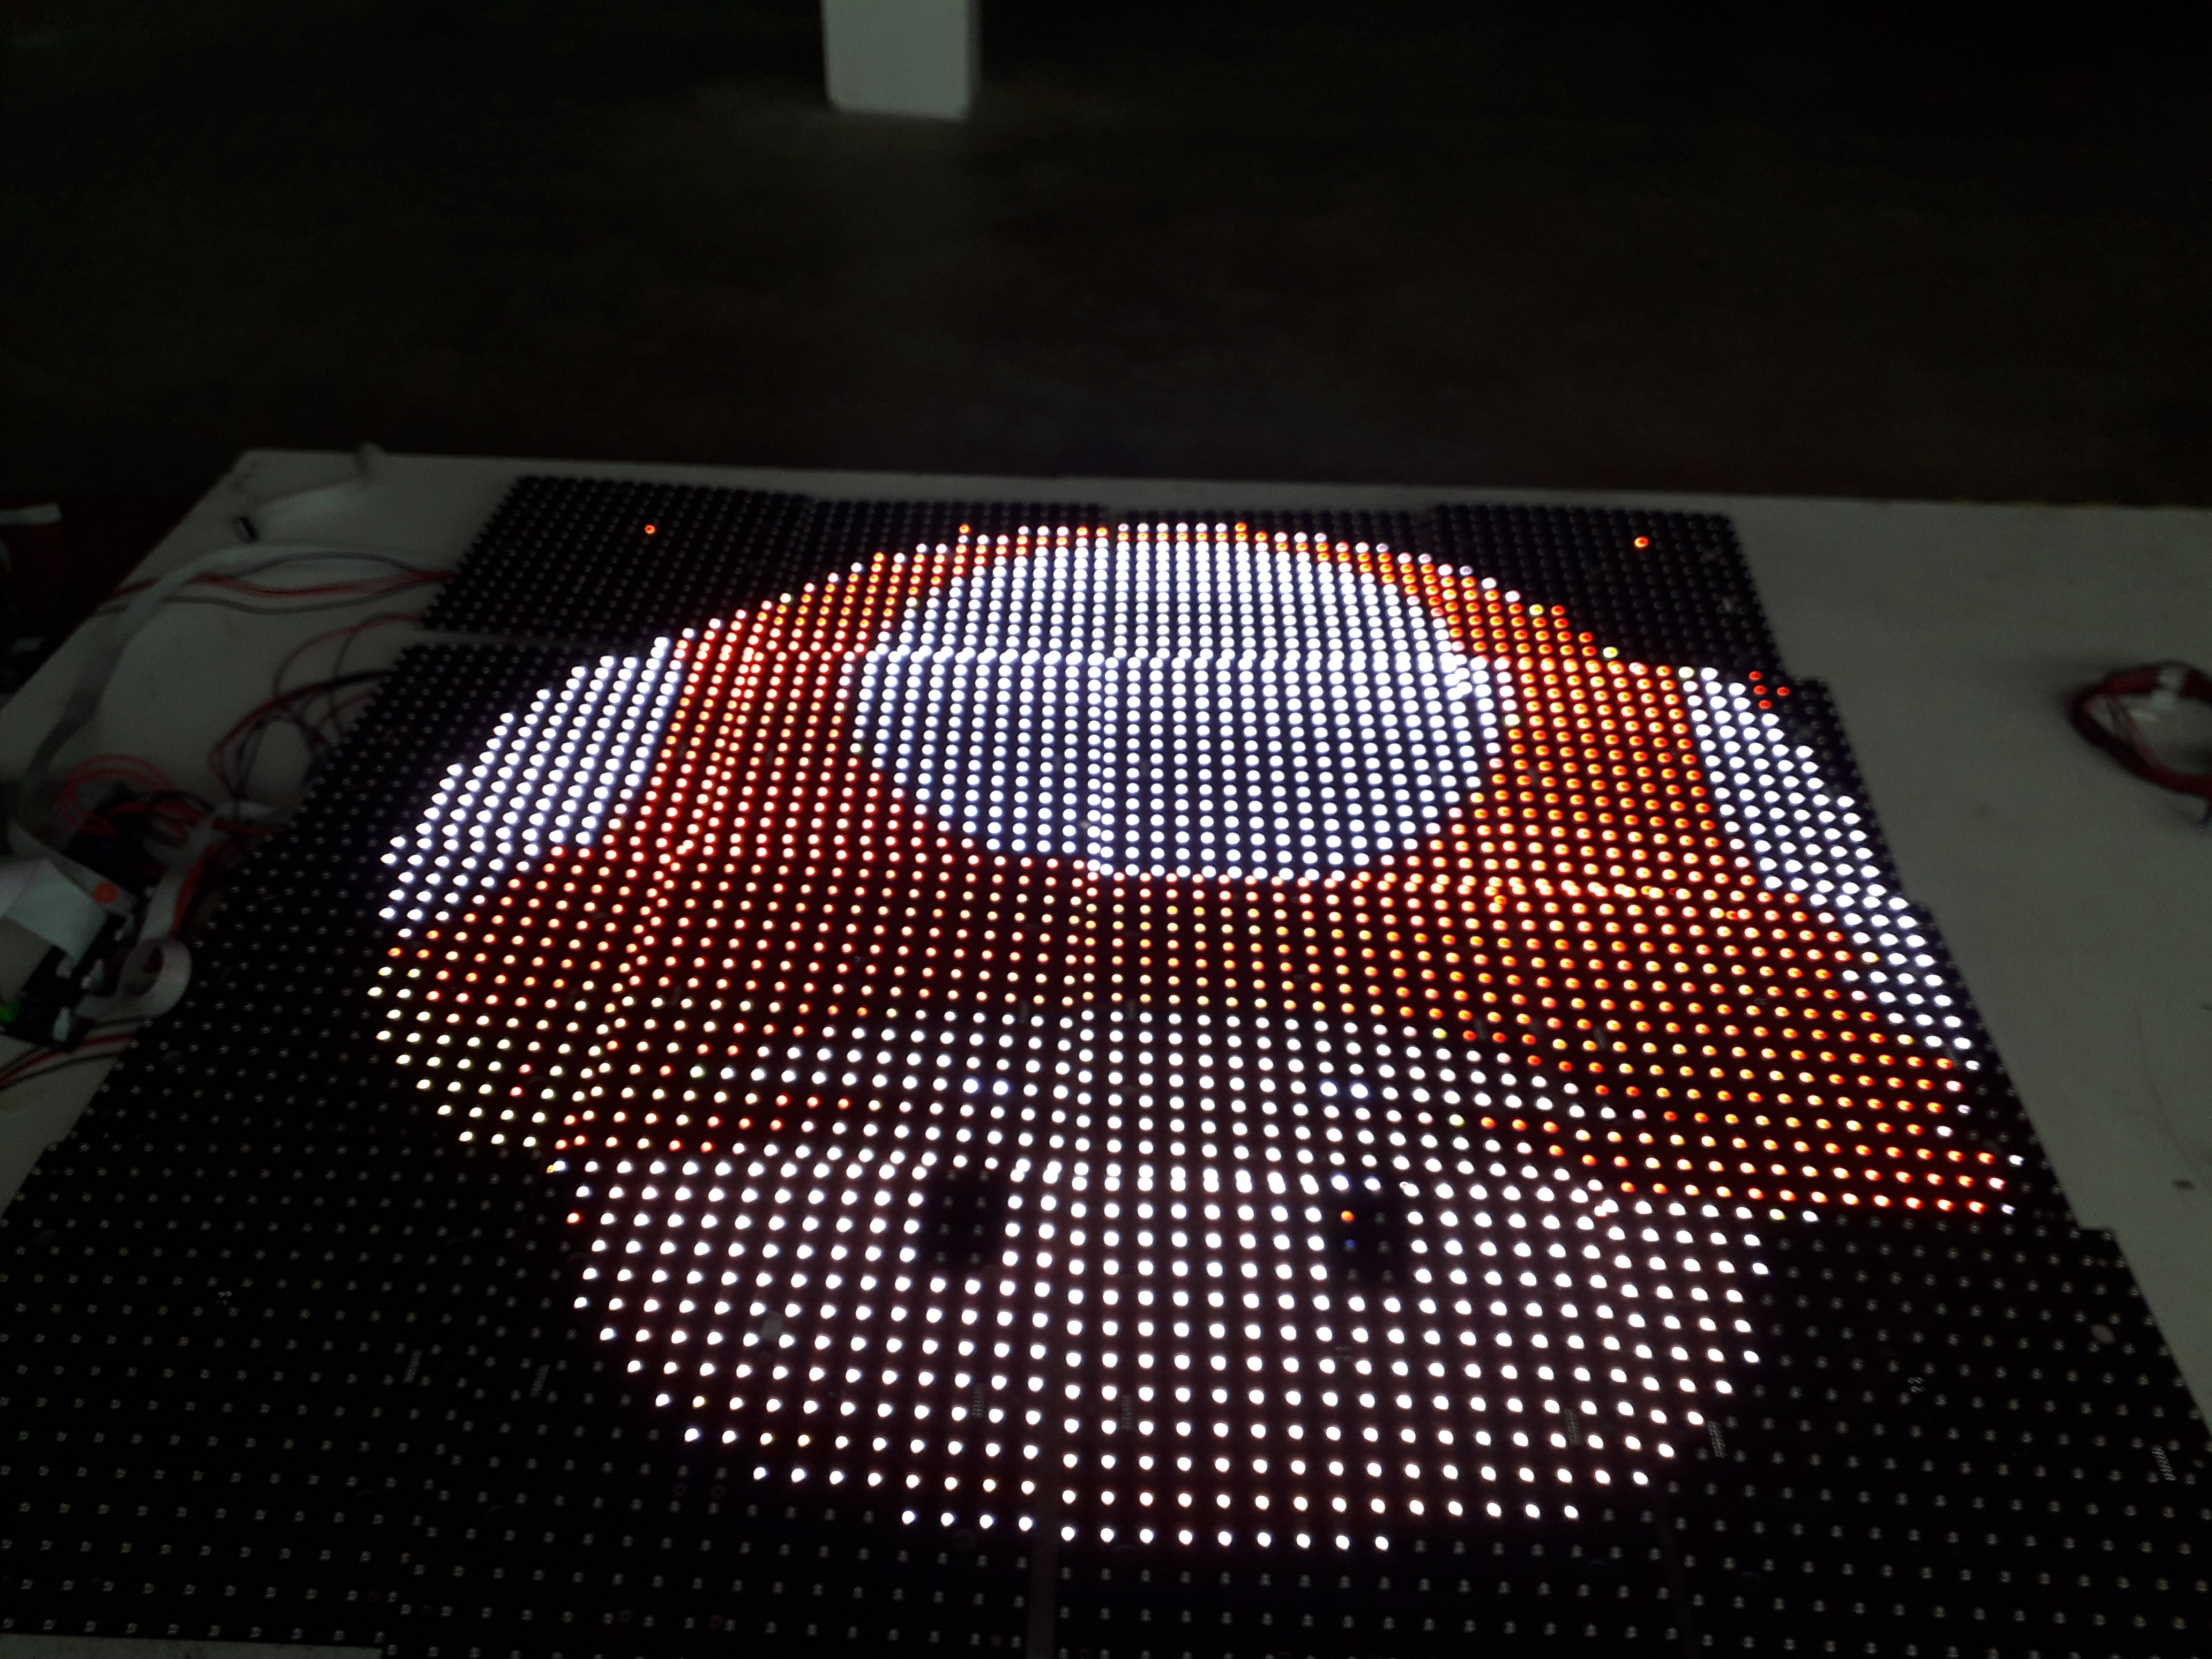
\includegraphics[scale=0.1]{Figures/matriz4x4.jpg} 
	\caption{Ensayo de sistema sobre mesa de trabajo.}
	\label{fig: matriz4x4}
\end{figure}

\subsection{Ensayo de matrices sobre estructura metálica a nivel de piso}
Para realizar este ensayo se ensambló un arreglo de matrices de LEDs en la estructura metálica a nivel de piso. En la figura \ref{fig: matrizestructuraparcial} se puede apreciar los resultados de este ensayo. Este ensayo fue necesario debido a que cuando se realizaron los ensayos sobre la mesa de trabajo no se podían apreciar los resultados con claridad. Esta prueba sirvió para pulir detalles de la APP de escritorio. También se pudieron detectar y corregir errores en el despliegue de la imagen.

\begin{figure}[htpb]
	\centering
	\includegraphics[scale=0.1]{Figures/matrizsobreestructura.jpg} 
	\caption{Ensayo de sistema sobre estructura metálica.}
	\label{fig: matrizestructuraparcial}
\end{figure}

\subsection{Pruebas de pantalla completa sobre nivel de piso}
Para realizar este ensayo se ensambló la pantalla completa. En las figuras \ref{fig: pantallacompletasobrepiso1} y \ref{fig: pantallacompletasobrepiso2} se muestran los resultados de estos ensayos. Estos ensayos sirvieron para comprobar que las señales de control de las matrices LED no eran afectadas por el tamaño de la pantalla. La imágenes desplegadas en la pantalla fueron las esperadas.

\begin{figure}[htpb]
	\centering
	\includegraphics[scale=0.6]{Figures/vmsfc8m.jpg} 
	\caption{Ensayo de pantalla completa a nivel de piso 1.}
	\label{fig: pantallacompletasobrepiso1}
\end{figure}



\begin{figure}[htpb]
	\centering
	\includegraphics[scale=0.6]{Figures/vmsfc8m1.jpg}
	\caption{Ensayo de pantalla completa a nivel de piso 2.}
	\label{fig: pantallacompletasobrepiso2}
\end{figure}
 


\section{Pruebas de campo}

Se instalaron varias pantallas en diferentes puntos de la ciudad de Guayaquil en la figura \ref{fig: mapa} se muestra la ubicación de las pantallas instaladas.

Desde la estación remota se enviaron mensajes a diferentes pantallas como se puede observar en las figuras \ref{fig: calle1}, \ref{fig: calle2}, \ref{fig: calle3} y \ref{fig: calle4}. Las imágenes se desplegaron de manera correcta logrando comprobar el funcionamiento correcto de todo el sistema en el lugar de instalación.
La pruebas fueron realizadas en solo cuatro pantallas debido a que las otras pantallas estaban energizadas pero no tenían conexión a la estación remota.


\begin{figure}[htpb]
	\centering
	\includegraphics[scale=0.6]{Figures/mapapantallas.png} 
	\caption{Ubicación de pantallas.}
	\label{fig: mapa}
\end{figure}




\begin{figure}[htpb]
	\centering
	\includegraphics[scale=3]{Figures/calle1.jpg} 
	\caption{Pantalla en vía 1.}
	\label{fig: calle1}
\end{figure}

\begin{figure}[htpb]
	\centering
	\includegraphics[scale=1.5]{Figures/calle2.jpg} 
	\caption{Pantalla en vía 2.}
	\label{fig: calle2}
\end{figure}

\begin{figure}[htpb]
	\centering
	\includegraphics[scale=2]{Figures/calle3.jpg} 
	\caption{Pantalla en vía 3.}
	\label{fig: calle3}
\end{figure}

\begin{figure}[htpb]
	\centering
	\includegraphics[scale=0.6]{Figures/calle4.jpg} 
	\caption{Pantalla en vía 4.}
	\label{fig: calle4}
\end{figure}